%%% Local Variables: 
%%% mode: latex
%%% TeX-master: "../KanjiHWR"
%%% End: 
\chapter{E-Learning}
\label{chap:elearning}
% xxx: s. 12 beachten: WICHTIG!
% S. 12: tilman sagt:
% Nicht Lernkonzepte vergleichen und evaluieren, 
% sondern sehen, was die Technik bietet und entsprechende use-cases darstellen.

\section{Introduction to E-Learning}
\label{sec:elearn:intro}

The term \emph{e-learning} refers to a number of different methods, concepts
and techniques. It is therefore difficult to confine the term sharply.
Thus, in literature, there are different definitions of what e-learning is
and what it is supposed to be.
\shortciteANP{Rosenberg2006} \citeyear{Rosenberg2006} defines e-learning as
follows:
  \begin{quote}
    \textbf{E-learning} is the use of Internet technologies to create and
    deliver a rich learning environment that includes a broad array of 
    instruction and information resources and solutions, the goal of which
    is to enhance individual and organizational performance.
  \end{quote}
\shortciteANP{Rosenberg2006} defines e-learning purely by terms of instruction
and information resources. Further, \emph{the use of Internet technologies} 
is seen as a necessary condition for e-learning. The definition does not 
take into account educational software.

\shortciteANP{Richert2007} \citeyear{Richert2007} critises the definition of
\shortciteANP{Rosenberg2006} because she sees no reason for such equality
of terms. She constitutes her view with the fact that electronic (learning) 
applications are not limited to the Internet. \shortciteANP{Richert2007} 
\citeyear{Richert2007} defines e-learning as:
  \begin{quote}
    Unter E-learning wird das computergestützte Lernen (vorwiegend von 
    Einzelpersonen) mit hypertextbasierten, multimedialen, interaktiven 
    Systemen verstanden, das zeit- und ortsunabhängig sowohl online als 
    auch offline erfolgen kann.
  \end{quote}
in English:
  \begin{quote}
    E-learning is defined as computer-aided learning (mainly by individuals)
    with hypertext- and multimedia-based interactive systems. The learning
    process can take place independent of time and location both online and 
    offline.
  \end{quote}
It is important to note that the term is broader than the definition of
\shortciteANP{Rosenberg2006}, but is restricted to \emph{learning systems}.
That means concretely that electronic media like dictionaries may be included
in e-learning systems as a tool, however, they can only form a part of a 
more general e-learning environment. Electronic media itself is not necessarily
understood as e-learning system.

%\section{E-Learning Methodology}
%\label{sec:elearn:methodology}

\section{Classification of E-Learning Systems} %was subsection of methodology
\label{sec:elearn:classification}

E-learning systems can be classified by their their degree of freedom for 
user interaction. On one end of the scale there are \emph{Drill-and-Practice} 
programs that do not allow for freedom of interaction. On the other end there 
are interactive programs allowing the user to interact and control the 
application. Judged by the definition of \shortciteANP{Richert2007} this 
classification does not seem very suitable~\shortcite{Richert2007}.

Another possiblility to classify e-learning systems is the the kind of storage
media used. This classification allows for a distinction between \emph{online} 
and \emph{offline} e-learning systems. \emph{Offline systems} are those systems
that are offered on passive storage media like floppy disk, CD-ROM.
Offline systems are usually called \emph{Computer Based Training} (CBS) systems.
\emph{Online systems} on the other hand are web server based systems that fall
under the category of \emph{Web Based Training} (WBS) 
systems~\shortcite{Richert2007}.

Additionally, \shortciteANP{Richert2007} \citeyear{Richert2007} defines
\emph{hybrid systems} that are CBT systems but use the Internet as a means of
communication with other learners.
Table~\ref{table:elearningsystems} shows the classification of e-learning systems
after~\shortcite{Richert2007}.
\begin{table}[htbp]
\begin{tabular}{|c|c|c|c|}
  \hline
  \multicolumn{2}{|c|}{} & \multicolumn{2}{|c|}{Using the WWW as storage medium} \\
  \cline{3-4}
  \multicolumn{2}{|c|}{} & Yes & No \\
  \hline
  \multirow{2}{*}{Using the Internet for communication} & No & WBT & CBT \\
  \cline{2-4}
   & Yes & Learning platforms & Hybrid CBT \\
  \hline
\end{tabular}
\caption{Classification of e-learning systems}
\label{table:elearningsystems}
\end{table}

\section{Technical Context of E-Learning}
\label{sec:elearn:technicalcontext}

\subsection{Multimedia Systems}
\label{sec:elearn:multimediasystems}

The term \emph{Multimedia} has several definitions. Simple versions of 
multimedia definitions state that multimedia refers to a combination of
different forms of information from several sources. Those forms can contain
textual information, graphic, video and audio. With a broad definition
of that kind any television news report could be regarded as multimedia.
\shortciteANP{Richert2007} \citeyear{Richert2007} understands \emph{multimedia}
more holistically than that. She sees multimedia as a technological concept 
that allows for the interaction of a user and a multiple media system.
More than one sensorial modality should be should be presented by the system.

\subsection{Classification of Interactivity}
\label{sec:elearn:interactivity}

\emph{Interactivity} can be defined in several steps. The concept of 
\emph{interaction} serves as a basis for the classification, because in a 
sociological sense there can, by definition, be no mutual interference
between man and machine. Interactivity in the sense of interaction comprises
the ability to access and control different functionalities of a software 
system~\shortcite{Richert2007}.

Six classes of interactivity can be described. They differ by their degree of
interaction between the user and a software system.
The gamut of interactivity is used to evaluate e-learning applications:
\begin{enumerate}
\item \textbf{View and absorb objects} \\
      The hypermedial components can be viewed and played by the user.
      The user can not further influence the components in any way.
\item \textbf{View and absorb multiple displays} \\
      Program components offer more than one display. For instance, a user
      could click on a picture and be shown a different one.
      No modification of components is possible.
\item \textbf{Varying the form of representation} \\
      On this level, users can gain the feeling they could actively influence
      the multimedia components. They can scale objects or view them from
      different perspectives. Users can influence the form of representation
      but not the content.
\item \textbf{Changing the content of a component - parameter or data 
      variation} \\
      Contents of a multimedia component are generated by the user. Users can
      input data or text. They can not change films or pictures.
      A usage example of that type could be the selection methods of statistics
      programs. Users can modify objects and the program yields different 
      results.
\item \textbf{Generating objects or the content of a representation} \\
      This mode of interaction is reached by applications that offer tools to
      create and change content. For example visualise thoughts with mindmaps,
      or render new forms and models.
\item \textbf{Constructive and manipulative actions through 
      situation-dependent feedback} \\
      On this level of interaction symbols can be manipulated and the result of
      the interpretation can be interpreted by the program.
      That allows for the generatoin of useful and context-sensitive feedback.
      User input can be evaluated by the application.
\end{enumerate}
The gamut is described after~\shortcite{Richert2007}.

\section{Pedagogical Context of E-Learning}
\label{sec:elearn:pedagogicalcontext}

The pedagogical context of e-learning is a crucial part of any e-learning
environment. The learning targets need to be defined and a conceptual design
of a software needs to be based on those.

\subsection{Learning}
\label{sec:elearn:learning}

The term \emph{learning} is of a complex nature. A definition of learning is
therefore never sharply confined. The definition of \emph{learning} by 
\shortciteANP{Lefrancois1994} \citeyear{Lefrancois1994} shows how broad
the term can be percieved:
\begin{quote}
  \emph{Lernen umfasst alle Verhaltensänderungen, 
        die aufgrund von Erfahrungen zustandekommen.}
\end{quote}
In English:
\begin{quote}
 Learning compasses all changes in behaviour that are based on experience.
\end{quote}
The changes in behaviour include those processes that do not aim at acquiring
information, but also those changes in behaviour of an unknown 
cause~\shortcite{Lefrancois1994}. According to~\shortcite{Richert2007},
this means the acquisition of competences of different kinds.

\subsubsection{Educational Objectives}
\label{sec:elearn:learningaims}

\paragraph{Cognitive learning targets} comprise all targets that include acquisition 
of knowledge. Knowledge can refer to both reproduction of content, but also 
acquiring the ability to solve problems. The area of cognitive learning targets
can be differentiated further.~\shortciteANP{Richert2007} \citeyear{Richert2007} 
distinguishes the acquisition of:
\begin{itemize}
  \item \textbf{Declarative knowledge} or \textbf{factual knowledge}. Knowledge
        that can be categorised as \emph{knowing that} as opposed to 
        \emph{knowing how}.
  \item \textbf{Procedural knowledge} or \textbf{dynamic knowledge}. Knowledge
        that contains approaches to problems and their resolution procedures.
        Procedural knowledge can be seen as a series of declarative inventory
        of knowledge, nevertheless it can be categorised as \emph{knowing how}.
        The distinction to the regular ability of a human to solve problems lies
        in the fact that declarative knowledge is needed in order to solve
        specific types of problems. For instance, in order to be able to 
        successfully use a map for navigating, a human needs to know that a 
        certain object is a map, what the symbols on the map mean and 
        where or what the four cardinal points are.
  \item \textbf{Contextual knowledge}. Knowledge that contains application
        situations. This category is centred around \emph{when and where} to
        apply knowledge. What abilities and which factual knowledge can be
        used in which situations?
\end{itemize}

\paragraph{Affective learning targets} are educational objectives that aim at changing
behaviour. It is difficult to actualise affective learning targets by cognitive
learning only. In order to achive affective learning targets, feelings, 
evaluations and attitudes of humans need to be taken into account. In learning 
situations at school often personal enthusiasm, credibility and charisma of 
the teacher play a role~\shortcite{Richert2007}.

\paragraph{Psychomotoric learning targets} is the class of learning targets that aim 
at the acquisition of manual abilities and motion sequences. That includes 
playing of musical instruments or using tools. Analogue to the procedural 
knowledge learning, theoretical knowledge about the objects involved is necessary
in order to achieve the psychomotoric abilities. That theoretical knowledge is
a necessary condition for the psychomotoric learning process, but it is not
sufficient, psychomotoric learning involves practising motoric 
sequences~\shortcite{Richert2007}.

\subsubsection{Self-Driven Learning}
\label{sec:elearn:selfdrivenlearning}

Learning is often seen as a behaviourist stimulus-recation process. Different 
views observe an active and constructive process. In the constructionist
view on learning there is a continuum from \emph{self-learning} to
\emph{autonomous learning}. \emph{Self-driven learning} can be classified
by that continuum.

\paragraph{Self-learning} defines a type of learning with a focus on the 
self-initiative and self-responsibility of a learner. 
\shortciteANP{Richert2007}~\citeyear{Richert2007} reports of the
opinion that it is impossible to not self-learn, because learning always
assumes the intention of the learner. This view conjectures that each learner 
has to accomplish the task of self-construction of knowledge. However,
self-learning defines solely the self-initiative of the learner, the learning
material is provided by an external source.

\paragraph{Autonomous learning} is distinct from self-learning in the way,
that it focuses on teacher-independent organisation of learning. 
While in self-learning, the learner can decide to learn, independently
of a teacher, in autonomous learning the learner is self-responsible 
for defining learning targets and has an analytical view on the 
learning process~\shortcite{Richert2007}.

\paragraph{Self-driven learning} is a type of learning that can be seen somewhere
on the continuum from self-learning to autonomous learning. In self-driven 
learning the learner is given all instructions and decisions concerning the
learning process in the learning materials. The self-direction is therefore 
limited to the location and the time of learning~\shortcite{Richert2007}.

\subsection{Intelligent Tutorial Systems}
\label{sec:elearn:intelligenttutorialsystems}

Intelligent tutorial systems fall under the paradigm of cognitive learning.
The general scheme of such a system is depicted after~\shortcite{Richert2007} in 
figure~\ref{fig:tutorialsystems}. 
The declarative knowledge of a system is stored in the expert module. 
The student module holds information about the learning progress and the
course module holds the lessons of the application.
The communication module interacts with the learner.
\begin{figure}[htbp]
\begin{center}
\includegraphics[scale=0.5]{images/E-Learning/tutorialSystems.png}
\caption{General scheme of intelligent tutorial systems}
\label{fig:tutorialsystems}
\end{center}
\end{figure}

\section{E-Learning of Languages}
\label{sec:elearn:elearningoflanguages}
strengthening of competences (s.96)
richert: s. 95
97ff

\section{E-Learning of Japanese Script}
\label{ser:elearn:elearningofjapanesescript}

\subsection{Conceptual Issues for E-Learning of Kanji}
\label{sec:elearn:conceptualissuesforelearningofkanji}

\subsection{Classification of a Kanji Teaching Application}
\label{sec:hwre:classificationofakanjiteachingapplication}




%\section{Japanese E-Learning Software}
%put all your bashing and criticism here
%e-learning software can be found here. zitiert von stahlmann.
%siehe wortsalat
%http://www.geotechnics.ch/Fritz/Schule/pages/lernsw/LernSW.htm


computer assisted language learning:
\shortcite{Bailey2009} %siehe seite 34 im heft

\shortcite{Zimmer2009}Bildung durch e-learning. allgemeine aspekte
\shortcite{Stahlmann2004} spezielle aspekte bezueglich han-trainer pro
\shortcite{Hettinger2008} wie kann man e-learning in der schule einsetzen?
e-learning: grundlagen, modelle, perspektiven

\shortcite{Richert2007} breite einfuehrung in e-learning theorie.

\shortcite{Seel2009} sehr breite allgemeine einfuehrung ins online-lernen
\shortcite{Ivashin2009}kritik an der technischen dominanz in elektronisch
unterstuetzten lern- und lehrprozessen.

\shortcite{Stark2002} comparison of two e-learning apps.
